\documentclass[twocolumn]{article}

\usepackage[utf8]{inputenc} %Para configuración de caracteres
\usepackage[spanish]{babel} %Para configuración de idioma
\usepackage{graphicx}
\usepackage{amsmath}
\usepackage{amsfonts}
\usepackage{float}
\let\olditemize\itemize
\def\itemize{\olditemize\itemsep=0pt } %%Reducir espacio itemize
\usepackage{xcolor}
\usepackage{anysize} %Para usar márgenes
\marginsize{2cm}{2cm}{1cm}{2cm} %{izquierda}{derecha}{arriba}{abajo}.
\usepackage{listings}
\usepackage{listingsutf8}
\lstset{ %
  basicstyle=\footnotesize,           % the size of the fonts that are used for the code
  numberstyle=\footnotesize,          % the size of the fonts that are used for the line-numbers
  numbersep=4pt,                  % how far the line-numbers are from the code
  backgroundcolor=\color{white},      % choose the background color. You must add \usepackage{color}
  breaklines=true,                % sets automatic line breaking
  breakatwhitespace=false,        % sets if automatic breaks should only happen at whitespace
  title=\lstname,                   % show the filename of files included with \lstinputlisting;{}
  extendedchars=false,
  inputencoding=utf8, 
}

\title{	
\includegraphics[scale=0.2]{univalle.jpg} \\ Proyecto Final \\FUNDAMENTOS DE ANÁLISIS Y DISEÑO DE ALGORITMOS}
\author{Carlos Andres Delgado S, Ing \footnote{ carlos.andres.delgado@correounivalle.edu.co }}
\date{Mayo de 2017}

\begin{document}
\maketitle

Este taller se puede trabajar en grupos de hasta 3 personas. Entregue el código fuente solicitado y elabore un informe en formato PDF con la información solicitada en este proyecto.

\section{El problema}

Como si no fueran lo suficientemente complejos los Sudokus, en Julio de 2009, la revista Games Magazine describió una variante del juego que combina el Sudoku y el Dominó llamado \textbf{Su-Domino-Ku}. El juego tiene la forma de un Sudoku normal, es decir, una grilla de $9 9$ que debe ser llenada usando solo los dígitos del $1$ al $9$. En una solución exitosa:

\begin{itemize}
	\item Cada fila tiene que contener todos los  del 1 al 9.
	\item Cada columna tiene que contener todos los digitos del 1 al 9.
	\item Cada región de 3 x 3 tiene que contener todos los dígitos del 1 al 9.
\end{itemize}

Pero para un Su-Domino-ku, nueve celdas son inicializadas con los números del 1 al 9. Esto deja 72 celdas sin inicializar. Ellas deben ser llenadas usando un conjunto de 36 piezas de dominó. El conjunto incluye un dominó para cada posible par de números únicos desde el 1 hasta el 9 (Ejemplo: $1+2, 1+3, 1+4, 1+5, 1+6, 1+7, 1+8, 1+9, 2+3, 2+4, 2+5, . . . $). Note que no existen las piezas simétricas $1+2$ y $2+1$ en el conjunto, ya que cada una de estas piezas puede convertirse en la otra rotándola. Además note que los dominós pueden cruzar el límite de las regiones $3 x 3$ (como lo hace el dominó $9+2$ del siguiente ejemplo). Por ejemplo, la siguiente figura \ref{fig:inicial} muestra un juego en su estado inicial y la figura \ref{fig:final} la única forma de completar el rompecabezas:


\begin{figure}[H]
	\centering
	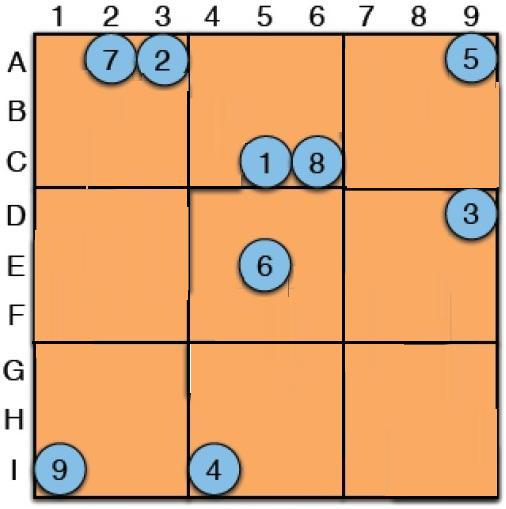
\includegraphics[scale=0.4]{Domino1.jpg}
	\caption{Su-Domino-ku en su estado inicial}
	\label{fig:inicial}
\end{figure}

\begin{figure}[H]
	\centering
	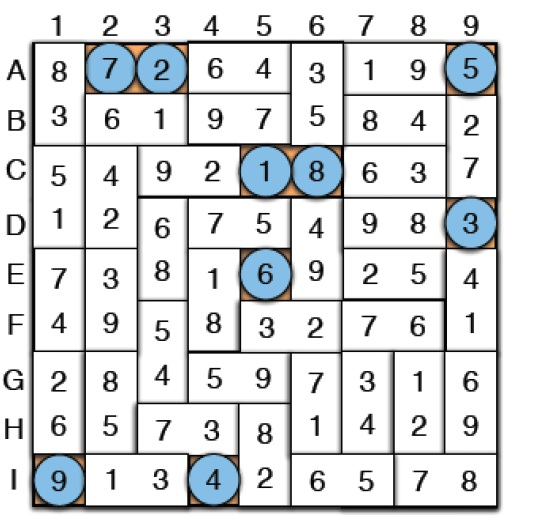
\includegraphics[scale=0.4]{Domino2.jpg}
	\caption{Su-Domino-ku en su estado final}
	\label{fig:final}
\end{figure}

Se espera que a partir de una entrada dada, el programa calcule la solución del Su-Domino-Ku. Las fichas disponibles se muestran en la siguiente figura:

\begin{figure}[H]
	\centering
	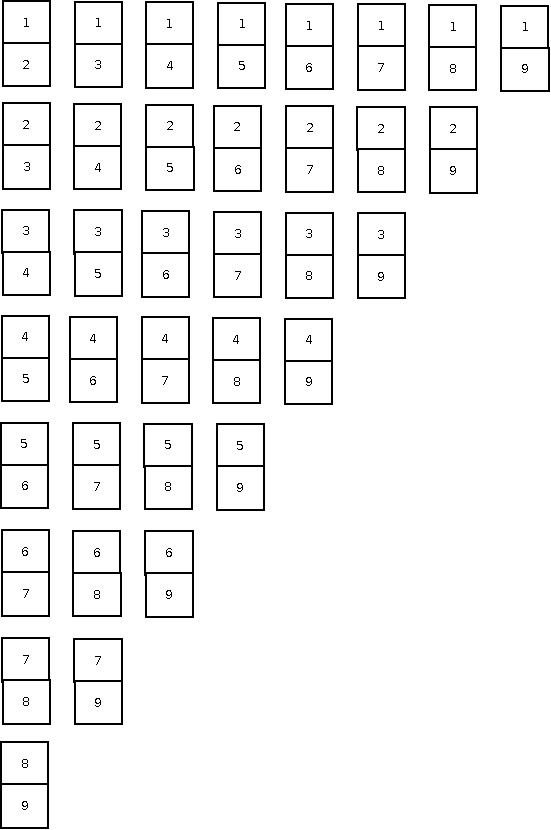
\includegraphics[scale=0.45]{domino-set.jpg}
	\label{fig:fichasDomino}
	\caption{Fichas de dominó}
\end{figure}

Recuerde la rotación de una ficha:

\begin{figure}[H]
	\centering
	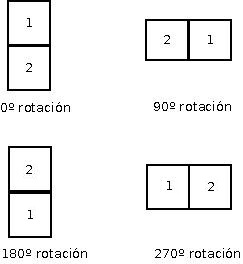
\includegraphics[scale=0.6]{Rotaciones.jpeg}
	\caption{Rotaciones de una ficha de dominó}
	\label{fig:dominoRotacion}
\end{figure}

\section{Solución}

Para el desarrollo de este proyecto se pueden escoger el ambiente de desarrollo y el lenguaje de
programación en el que va a trabajar.\\\\
El estado inicial del tablero se ingresa en un archivo de siguiente forma:

\begin{itemize}
	\item {9 filas, donde cada final tiene el siguiente formato:
		\begin{itemize}
			\item Primera columna indica el valor a insertar.
			\item El número de la fila donde va el valor.
			\item El número de la columna donde va el valor.
		\end{itemize}			
	}
	\item La décima fila contiene el número de fichas ya insertadas en el tablero. Este valor es mayor o igual $0$. En el caso que es $0$ no hay fichas en el tablero.
	\item Las siguientes filas, indican en sus dos primeras columnas la ficha de la figura \ref{fig:fichasDomino}, en la tercera su rotación y en las dos siguientes su posición inicial en el tablero.
\end{itemize}

Para el estado inicial mostrado en la figura \label{ref:inicial} la entrada tendría la siguiente forma:

\begin{lstlisting}
1 3 5
2 1 3
3 4 9
4 9 4
5 1 9
6 5 5
7 1 2
8 3 6
9 9 1
10
1 6 90 2 2
4 8 90 2 8
2 7 0 2 9
2 9 90 3 4
6 8 0 3 3
4 7 180 6 1
2 3 90 6 6
6 7 90 6 8
5 9 270 7 5
7 8 270 9 9
\end{lstlisting}

La salida se debe mostrar o almacenar en un archivo de salida de la siguiente forma:

\begin{itemize}
	\item 9 filas, con cada una 9 columnas que muestra la solución final del Su-Domino-Ku.
	\item La décima fila es un espacio en blanco.
	\item De la 11 fila en adelante con las figuras utilizadas, indicando su valor, rotación y posición. En caso de que la ficha no esté siendo utilizada en la solución, no se coloca rotación ni posición de la ficha.
\end{itemize}

Un fragmento de la salida del algoritmo se puede ver a continuación.

\begin{lstlisting}
8 7 2 6 4 3 1 9 5
3 6 1 9 7 5 8 4 2
5 4 9 2 1 8 6 3 7
1 2 6 7 5 4 9 8 3
7 3 8 1 6 9 2 5 4
4 9 5 8 3 2 7 6 1
2 8 4 5 9 7 3 1 6
6 5 7 3 8 1 4 2 9
9 1 3 4 2 6 5 7 8

1 2 0 7 8
1 3 270 9 3
1 4 180 5 9
1 5 180 1 3
1 6 180 2 2
1 7 180 7 6
1 8 0 5 4
1 9 90 1 8
...
\end{lstlisting}

\section{Criterios de evaluación}

Se deben implementar dos soluciones utilizando técnicas de programación diferentes:
Programación Dinámica y Programación Voraz.

\begin{itemize}
	\item Se debe documentar cada una de las soluciones escogidas, explicando la lógica de solución.
	\item Justificación de las estructuras de datos utilizadas en su solución.
	\item Se debe estimar la eficiencia en tiempo de ejecución de los dos algoritmos implementados.
	\item Se deben presentar las conclusiones del trabajo desarrollado.
	\item Este proyecto debe ser sustentado. La nota de sustentación va entre 0 y 1 es individual y su nota final se calcula multiplicando este factor por la nota obtenida en el proyecto.
\end{itemize}

Los criterios de evaluación son:

\begin{enumerate}
	\item \textbf{(30 \%)} Planteamiento completo de la solución dinámica
	\begin{enumerate}
		\item Caracterización de la estructura optima
		\item Definición recursiva del valor de una solución óptima
		\item Calculo de una solución óptima de manera Bottom-up
		\item Construcción de la solución óptima a partir de la información calculada
		\item Análisis de complejidad
	\end{enumerate}
	\item \textbf{(30\%)} Planteamiento de la solución voraz y su análisis de complejidad.
	\item \textbf{(15\%)} Redacción y estructura del informe. Incluya conclusiones, las cuale sno pueden ser cosas del marco teórico
	\item \textbf{(25\%)} Implementación. Es de aclarar que debe cumplir:
	\begin{itemize}
		\item Carga de entradas. El usuario puede especificar el archivo que puede cargar
		\item Implementación de estrategia voraz
		\item Implementación de estrategia de programación dinámica
		\item Desplegar al usuario información sobre la solución al problema (tablero)
		\item Desplegar al usuario información sobre la solución al problema (ingreso de fichas)
	\end{itemize}

\end{enumerate}



\end{document}